\section{Data}
According to the objective of our project, we require data for our analysis. Our data is derived from our online survey conducted over a week. All collected data is accessible only to authorized research team members.
    \subsection{Attributes Identification and Selection}
    Initially, we brainstorm and identify key attributes which will be included in our analysis such as user demographics, user behavior and user preferences. After discussing their relevance and potential impact on the user’s movie genre preferences, we eventually determine seven key attributes essential for our analysis: age, gender, working/learning area, preferred film genre, factor influencing genre choice, frequency of movie watching, source of film viewing.
            
        \subsection{Data Collection}
        \begin{itemize}
            \item \textbf{Step 1: Create a survey}\\
            We create a survey titled ‘Movie Genre Preferences’ to collect data via Google Forms. In the form, we focus on seven key attributes that we determined before. (as discussed in Section 2.1).
            \begin{figure}[H]
                \centering
                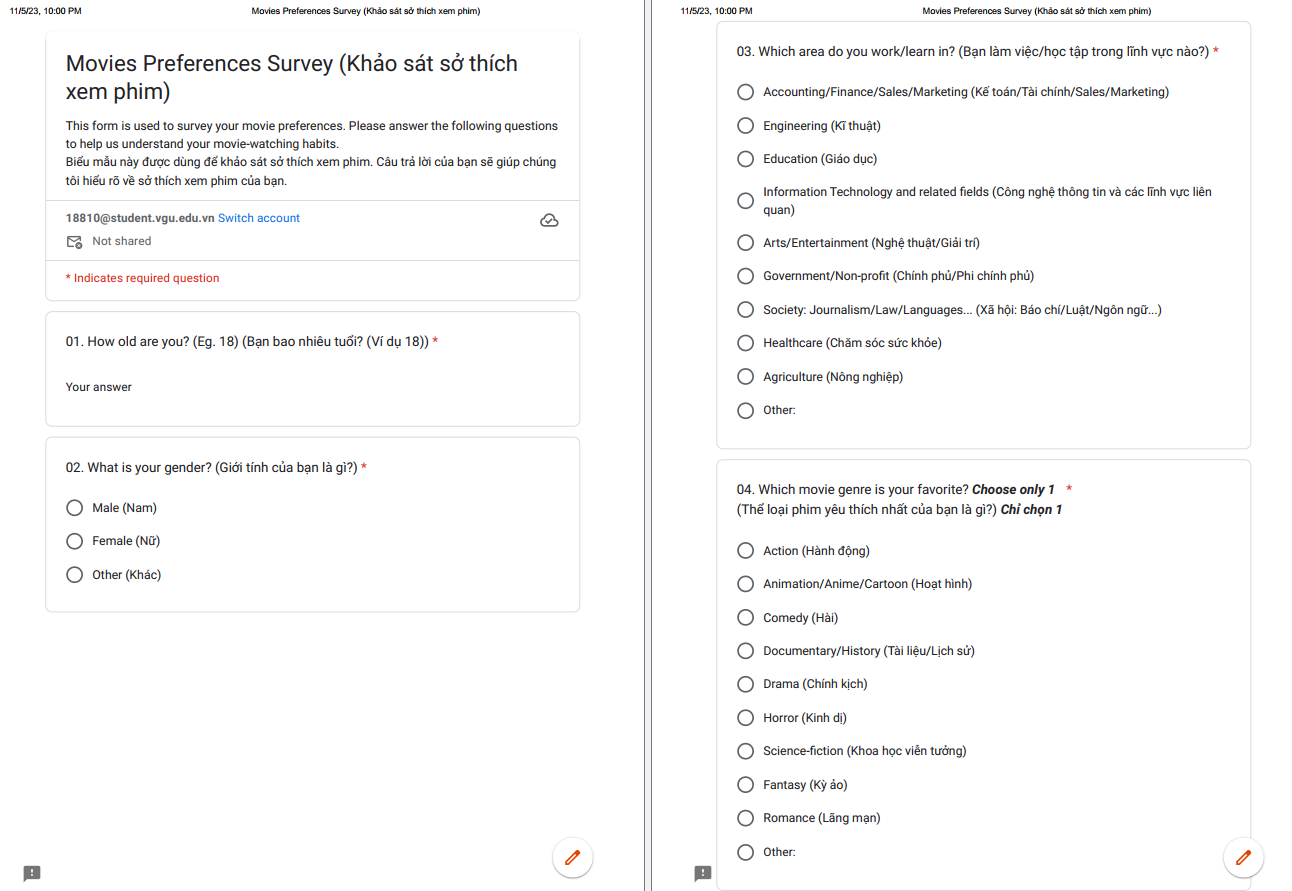
\includegraphics[scale=0.5]{graphics/data/Survey1.png}
                \caption{Movie genre preferences survey image (1)}
            \end{figure}
            
            \begin{figure}[H]
                \centering
                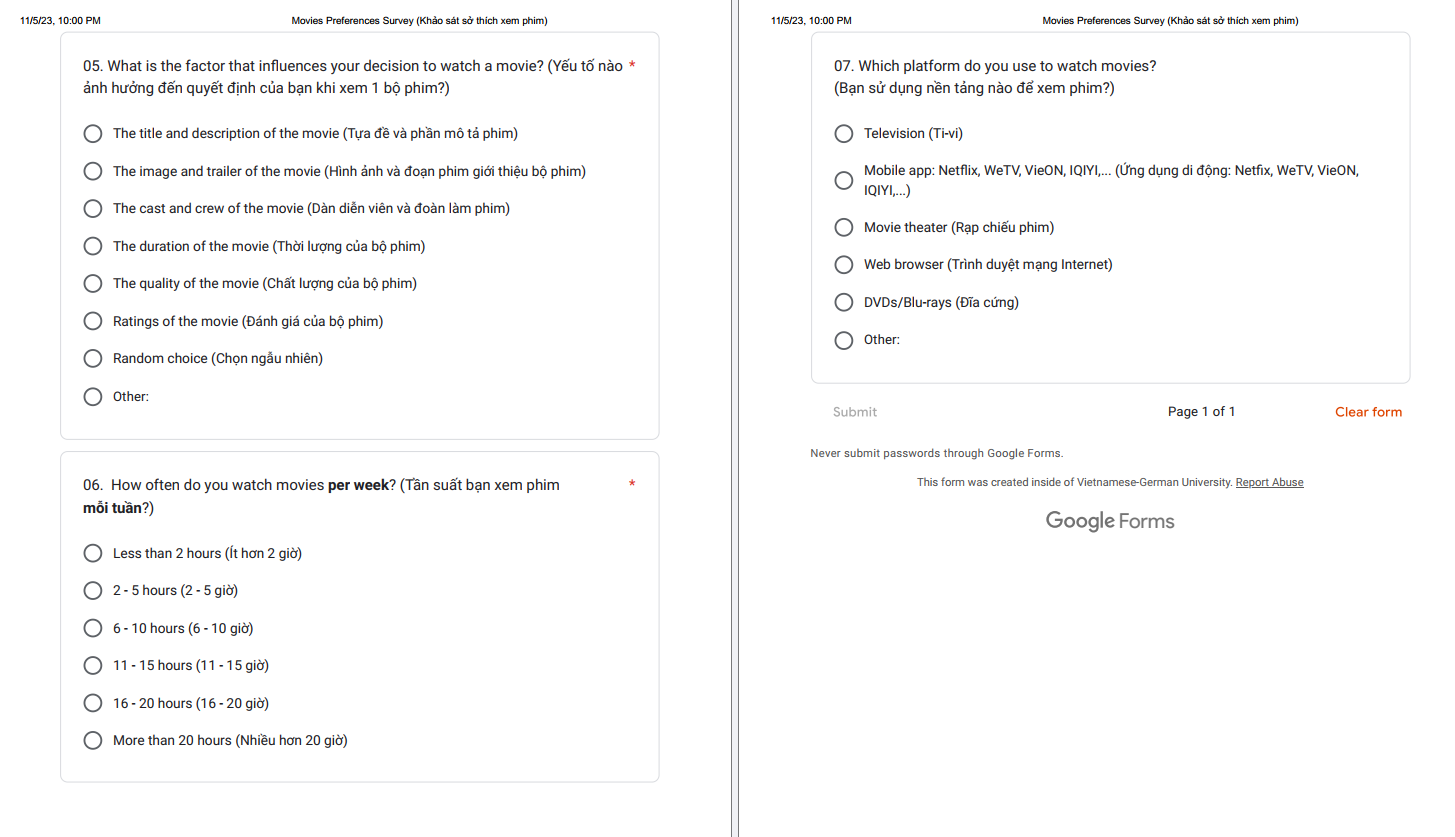
\includegraphics[scale=0.5]{graphics/data/Survey2.png}
                \caption{Movie genre preferences survey image (2)}
            \end{figure}
            
            \item \textbf{Step 2: Publish survey and receive responses}\\
            After completing the form, we distribute it to individuals, specifically targeting those aged 16 and above. Subsequently, we received a total of 118 responses from the survey. \\
            Here is an image of the responses list:
                \begin{figure}[H]
                    \centering
                    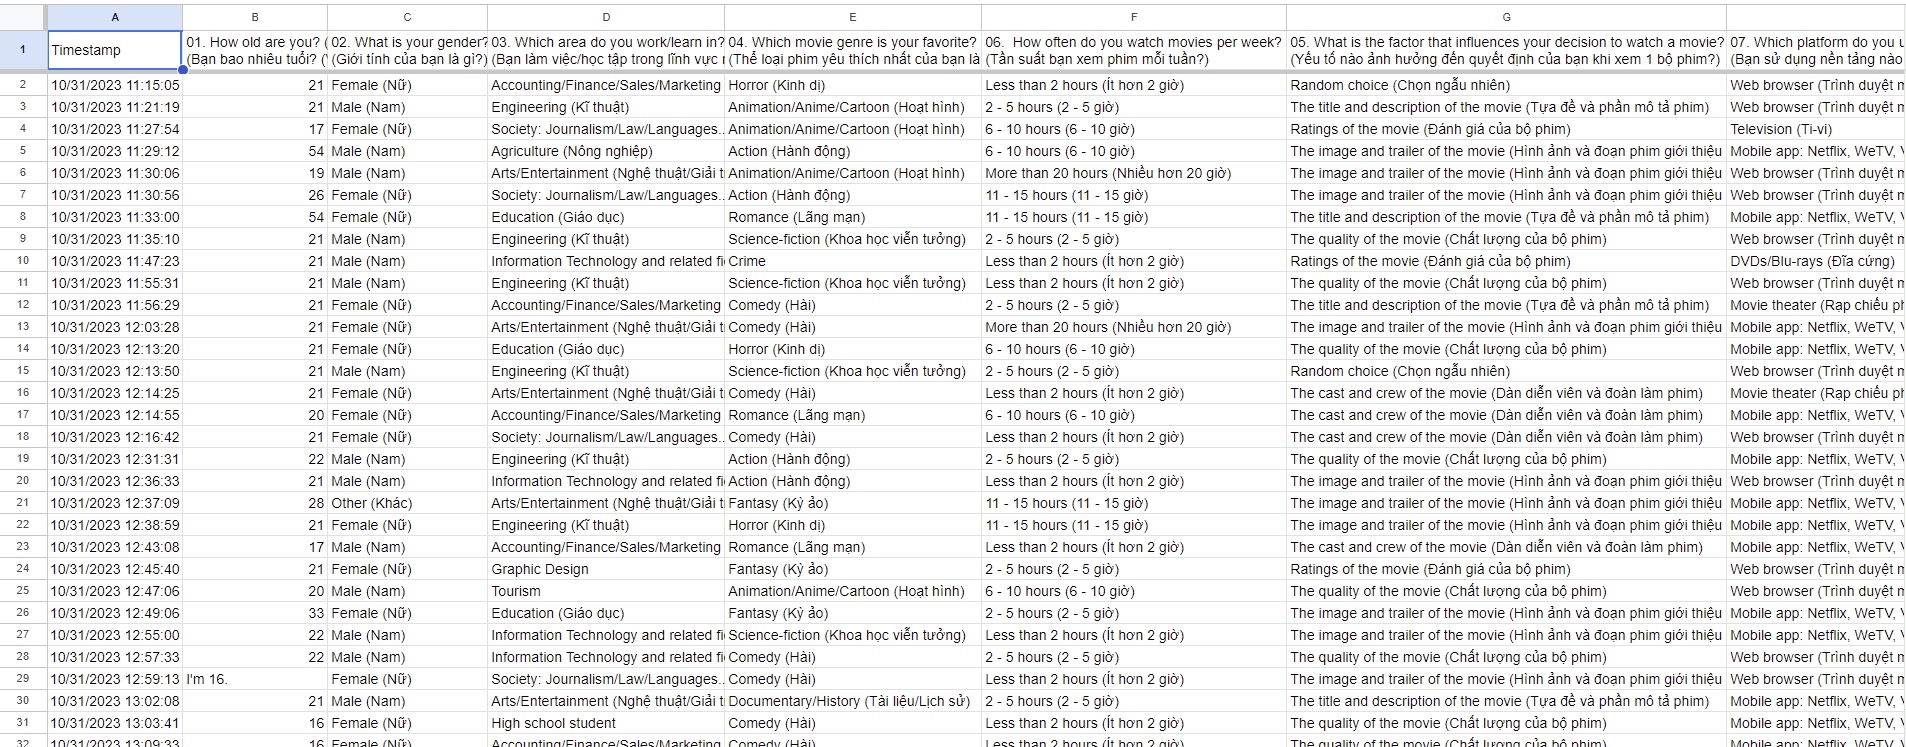
\includegraphics[scale=0.4]{graphics/data/dataResponses1.png}
                    \caption{Image of the responses list}
                \end{figure}
        \end{itemize}
        
    \subsection{Data Preparation}
   This process is crucial in minimizing the potential for errors and inaccuracies that may arise during our data processing stage. By ensuring the data is accurately prepared and processed, we can enhance the reliability and validity of our analysis.
    
    With a dataset of 118 responses, we come to the first crucial step for our data analysis: cleaning data.
                \begin{itemize}
                    \item In terms of attributes, we convert them from question format to word/phrase format:
                        \begin{figure}[H]
                            \centering
                            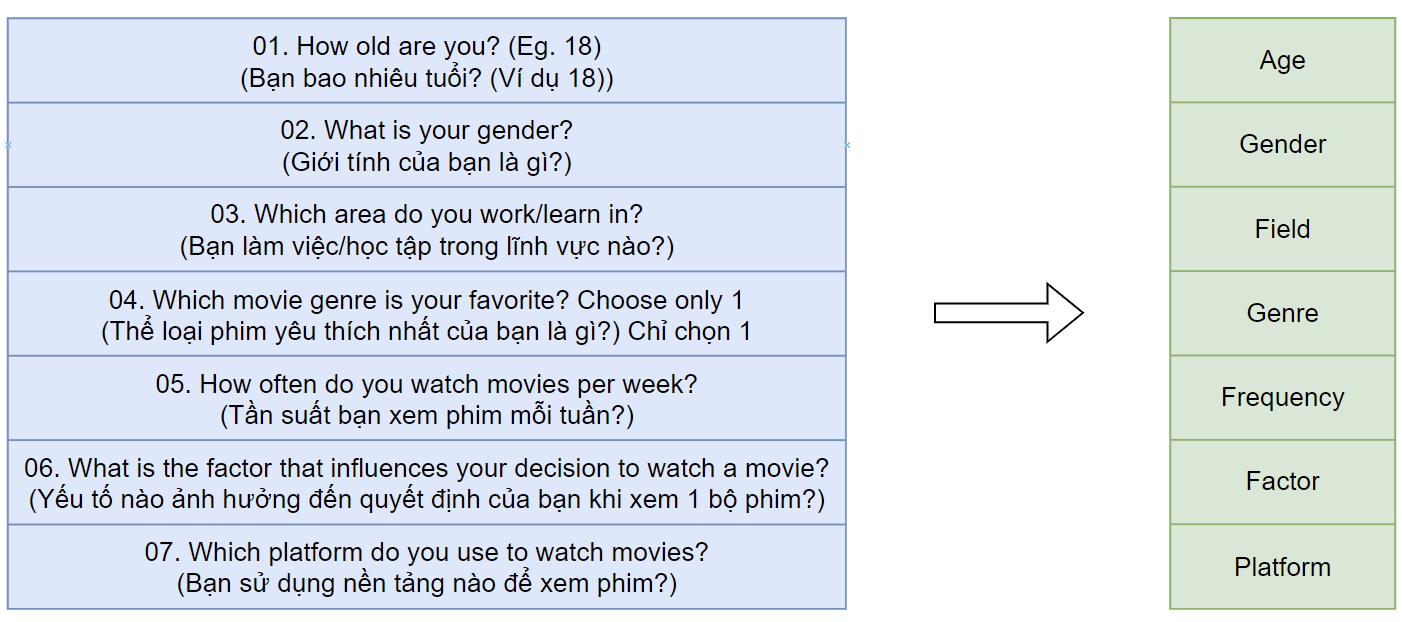
\includegraphics[scale=0.45]{graphics/data/questiontophrase1.png}
                            \caption{Image of attributes before and after}
                        \end{figure}
                    
                    \item We also substitute long words/phrases with shorter ones:
                         \begin{figure}[H]
                            \centering
                            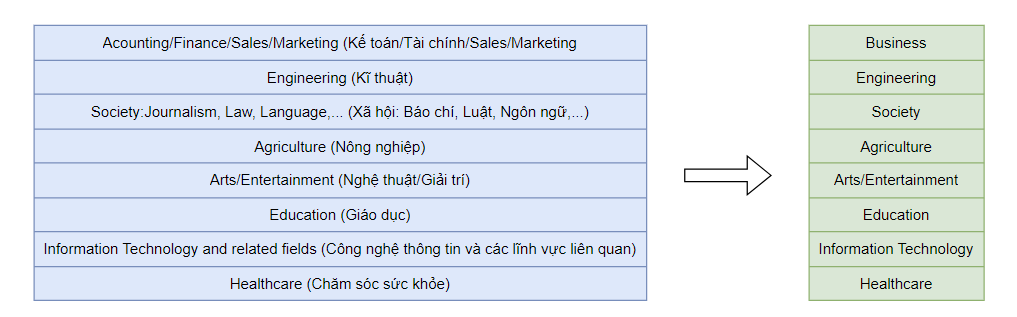
\includegraphics[scale=0.65]{graphics/data/substi.png}
                            \caption{Image of the data before and after substitution}
                        \end{figure}

                    \item Regarding working/learning area,  we decided to combine "real estate" as a part of "business":
                        \begin{figure}[H]
                            \centering
                            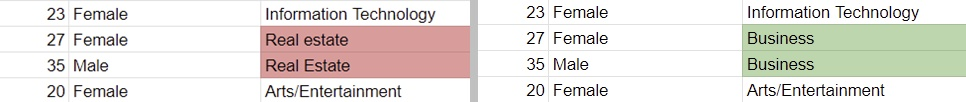
\includegraphics[scale=0.5]{graphics/data/realestate_business.jpg}
                            \caption{Image of the data before and after combination}
                        \end{figure}
                    
                    \item We adjust responses that are not in the correct format into our anticipated format:
                        \begin{figure}[H]
                            \centering
                            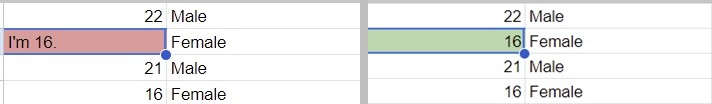
\includegraphics[scale=0.5]{graphics/data/Wrongformat3.jpg}
                            \caption{Image of the data before and after}
                        \end{figure}
                        
                    \item We remove responses that deviate from our expected range of values:
                        \begin{figure}[H]
                            \centering
                            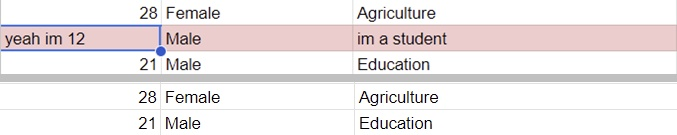
\includegraphics[scale=0.6]{graphics/data/eliminate3.jpg}
                            \caption{Image of the data example before and after elimination}
                        \end{figure} 

                    \item The entry “housewife” does not correspond to a specific work or learning area. Therefore, we exclude it from our dataset:
                        \begin{figure}[H]
                            \centering
                            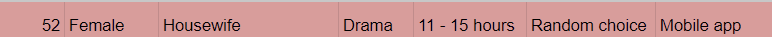
\includegraphics[scale=0.75]{graphics/data/housewife.png}
                            \caption{Image of the entry "housewife"}
                        \end{figure} 
                    After the data cleaning process, we obtain the final dataset. This dataset has the correct format, concise words/phrases, and values within an appropriate range for all attributes, making it suitable for our analysis.
                    \begin{figure}[H]
                        \centering
                        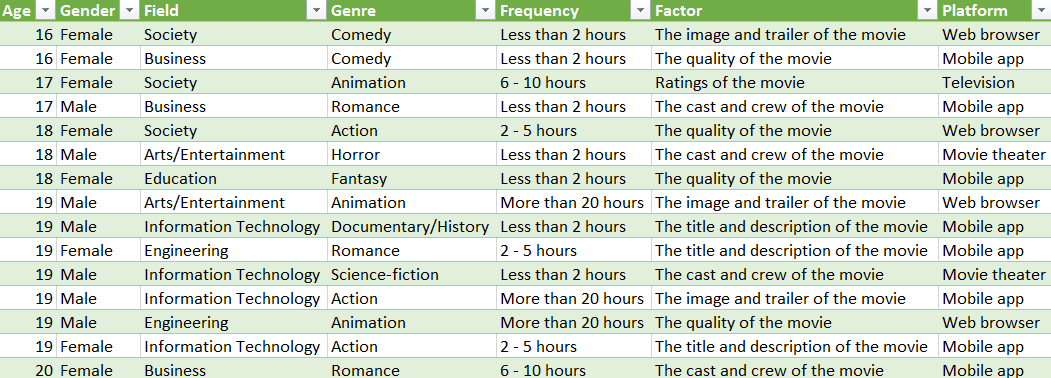
\includegraphics[scale=0.65]{graphics/data/finaldata.png}
                        \caption{Image of the final data after data cleaning process}
                    \end{figure} 
            In the next step, we apply the hierarchical clustering method to our final dataset, using dummy variables and mixed-type variables.
                \end{itemize}